% Generated by Sphinx.
\def\sphinxdocclass{report}
\documentclass[letterpaper,10pt,openany,oneside]{sphinxmanual}
\usepackage[utf8]{inputenc}
\DeclareUnicodeCharacter{00A0}{\nobreakspace}
\usepackage[T1]{fontenc}
\usepackage[english]{babel}
\usepackage{times}
\usepackage[Bjarne]{fncychap}
\usepackage{longtable}
\usepackage{sphinx}
\usepackage{multirow}


\title{Timing Cuda Operations}
\date{July 21, 2014}
\release{}
\author{CSInParallel Project}
\newcommand{\sphinxlogo}{}
\renewcommand{\releasename}{}
\makeindex

\makeatletter
\def\PYG@reset{\let\PYG@it=\relax \let\PYG@bf=\relax%
    \let\PYG@ul=\relax \let\PYG@tc=\relax%
    \let\PYG@bc=\relax \let\PYG@ff=\relax}
\def\PYG@tok#1{\csname PYG@tok@#1\endcsname}
\def\PYG@toks#1+{\ifx\relax#1\empty\else%
    \PYG@tok{#1}\expandafter\PYG@toks\fi}
\def\PYG@do#1{\PYG@bc{\PYG@tc{\PYG@ul{%
    \PYG@it{\PYG@bf{\PYG@ff{#1}}}}}}}
\def\PYG#1#2{\PYG@reset\PYG@toks#1+\relax+\PYG@do{#2}}

\expandafter\def\csname PYG@tok@gd\endcsname{\def\PYG@tc##1{\textcolor[rgb]{0.63,0.00,0.00}{##1}}}
\expandafter\def\csname PYG@tok@gu\endcsname{\let\PYG@bf=\textbf\def\PYG@tc##1{\textcolor[rgb]{0.50,0.00,0.50}{##1}}}
\expandafter\def\csname PYG@tok@gt\endcsname{\def\PYG@tc##1{\textcolor[rgb]{0.00,0.25,0.82}{##1}}}
\expandafter\def\csname PYG@tok@gs\endcsname{\let\PYG@bf=\textbf}
\expandafter\def\csname PYG@tok@gr\endcsname{\def\PYG@tc##1{\textcolor[rgb]{1.00,0.00,0.00}{##1}}}
\expandafter\def\csname PYG@tok@cm\endcsname{\let\PYG@it=\textit\def\PYG@tc##1{\textcolor[rgb]{0.25,0.50,0.56}{##1}}}
\expandafter\def\csname PYG@tok@vg\endcsname{\def\PYG@tc##1{\textcolor[rgb]{0.73,0.38,0.84}{##1}}}
\expandafter\def\csname PYG@tok@m\endcsname{\def\PYG@tc##1{\textcolor[rgb]{0.13,0.50,0.31}{##1}}}
\expandafter\def\csname PYG@tok@mh\endcsname{\def\PYG@tc##1{\textcolor[rgb]{0.13,0.50,0.31}{##1}}}
\expandafter\def\csname PYG@tok@cs\endcsname{\def\PYG@tc##1{\textcolor[rgb]{0.25,0.50,0.56}{##1}}\def\PYG@bc##1{\setlength{\fboxsep}{0pt}\colorbox[rgb]{1.00,0.94,0.94}{\strut ##1}}}
\expandafter\def\csname PYG@tok@ge\endcsname{\let\PYG@it=\textit}
\expandafter\def\csname PYG@tok@vc\endcsname{\def\PYG@tc##1{\textcolor[rgb]{0.73,0.38,0.84}{##1}}}
\expandafter\def\csname PYG@tok@il\endcsname{\def\PYG@tc##1{\textcolor[rgb]{0.13,0.50,0.31}{##1}}}
\expandafter\def\csname PYG@tok@go\endcsname{\def\PYG@tc##1{\textcolor[rgb]{0.19,0.19,0.19}{##1}}}
\expandafter\def\csname PYG@tok@cp\endcsname{\def\PYG@tc##1{\textcolor[rgb]{0.00,0.44,0.13}{##1}}}
\expandafter\def\csname PYG@tok@gi\endcsname{\def\PYG@tc##1{\textcolor[rgb]{0.00,0.63,0.00}{##1}}}
\expandafter\def\csname PYG@tok@gh\endcsname{\let\PYG@bf=\textbf\def\PYG@tc##1{\textcolor[rgb]{0.00,0.00,0.50}{##1}}}
\expandafter\def\csname PYG@tok@ni\endcsname{\let\PYG@bf=\textbf\def\PYG@tc##1{\textcolor[rgb]{0.84,0.33,0.22}{##1}}}
\expandafter\def\csname PYG@tok@nl\endcsname{\let\PYG@bf=\textbf\def\PYG@tc##1{\textcolor[rgb]{0.00,0.13,0.44}{##1}}}
\expandafter\def\csname PYG@tok@nn\endcsname{\let\PYG@bf=\textbf\def\PYG@tc##1{\textcolor[rgb]{0.05,0.52,0.71}{##1}}}
\expandafter\def\csname PYG@tok@no\endcsname{\def\PYG@tc##1{\textcolor[rgb]{0.38,0.68,0.84}{##1}}}
\expandafter\def\csname PYG@tok@na\endcsname{\def\PYG@tc##1{\textcolor[rgb]{0.25,0.44,0.63}{##1}}}
\expandafter\def\csname PYG@tok@nb\endcsname{\def\PYG@tc##1{\textcolor[rgb]{0.00,0.44,0.13}{##1}}}
\expandafter\def\csname PYG@tok@nc\endcsname{\let\PYG@bf=\textbf\def\PYG@tc##1{\textcolor[rgb]{0.05,0.52,0.71}{##1}}}
\expandafter\def\csname PYG@tok@nd\endcsname{\let\PYG@bf=\textbf\def\PYG@tc##1{\textcolor[rgb]{0.33,0.33,0.33}{##1}}}
\expandafter\def\csname PYG@tok@ne\endcsname{\def\PYG@tc##1{\textcolor[rgb]{0.00,0.44,0.13}{##1}}}
\expandafter\def\csname PYG@tok@nf\endcsname{\def\PYG@tc##1{\textcolor[rgb]{0.02,0.16,0.49}{##1}}}
\expandafter\def\csname PYG@tok@si\endcsname{\let\PYG@it=\textit\def\PYG@tc##1{\textcolor[rgb]{0.44,0.63,0.82}{##1}}}
\expandafter\def\csname PYG@tok@s2\endcsname{\def\PYG@tc##1{\textcolor[rgb]{0.25,0.44,0.63}{##1}}}
\expandafter\def\csname PYG@tok@vi\endcsname{\def\PYG@tc##1{\textcolor[rgb]{0.73,0.38,0.84}{##1}}}
\expandafter\def\csname PYG@tok@nt\endcsname{\let\PYG@bf=\textbf\def\PYG@tc##1{\textcolor[rgb]{0.02,0.16,0.45}{##1}}}
\expandafter\def\csname PYG@tok@nv\endcsname{\def\PYG@tc##1{\textcolor[rgb]{0.73,0.38,0.84}{##1}}}
\expandafter\def\csname PYG@tok@s1\endcsname{\def\PYG@tc##1{\textcolor[rgb]{0.25,0.44,0.63}{##1}}}
\expandafter\def\csname PYG@tok@gp\endcsname{\let\PYG@bf=\textbf\def\PYG@tc##1{\textcolor[rgb]{0.78,0.36,0.04}{##1}}}
\expandafter\def\csname PYG@tok@sh\endcsname{\def\PYG@tc##1{\textcolor[rgb]{0.25,0.44,0.63}{##1}}}
\expandafter\def\csname PYG@tok@ow\endcsname{\let\PYG@bf=\textbf\def\PYG@tc##1{\textcolor[rgb]{0.00,0.44,0.13}{##1}}}
\expandafter\def\csname PYG@tok@sx\endcsname{\def\PYG@tc##1{\textcolor[rgb]{0.78,0.36,0.04}{##1}}}
\expandafter\def\csname PYG@tok@bp\endcsname{\def\PYG@tc##1{\textcolor[rgb]{0.00,0.44,0.13}{##1}}}
\expandafter\def\csname PYG@tok@c1\endcsname{\let\PYG@it=\textit\def\PYG@tc##1{\textcolor[rgb]{0.25,0.50,0.56}{##1}}}
\expandafter\def\csname PYG@tok@kc\endcsname{\let\PYG@bf=\textbf\def\PYG@tc##1{\textcolor[rgb]{0.00,0.44,0.13}{##1}}}
\expandafter\def\csname PYG@tok@c\endcsname{\let\PYG@it=\textit\def\PYG@tc##1{\textcolor[rgb]{0.25,0.50,0.56}{##1}}}
\expandafter\def\csname PYG@tok@mf\endcsname{\def\PYG@tc##1{\textcolor[rgb]{0.13,0.50,0.31}{##1}}}
\expandafter\def\csname PYG@tok@err\endcsname{\def\PYG@bc##1{\setlength{\fboxsep}{0pt}\fcolorbox[rgb]{1.00,0.00,0.00}{1,1,1}{\strut ##1}}}
\expandafter\def\csname PYG@tok@kd\endcsname{\let\PYG@bf=\textbf\def\PYG@tc##1{\textcolor[rgb]{0.00,0.44,0.13}{##1}}}
\expandafter\def\csname PYG@tok@ss\endcsname{\def\PYG@tc##1{\textcolor[rgb]{0.32,0.47,0.09}{##1}}}
\expandafter\def\csname PYG@tok@sr\endcsname{\def\PYG@tc##1{\textcolor[rgb]{0.14,0.33,0.53}{##1}}}
\expandafter\def\csname PYG@tok@mo\endcsname{\def\PYG@tc##1{\textcolor[rgb]{0.13,0.50,0.31}{##1}}}
\expandafter\def\csname PYG@tok@mi\endcsname{\def\PYG@tc##1{\textcolor[rgb]{0.13,0.50,0.31}{##1}}}
\expandafter\def\csname PYG@tok@kn\endcsname{\let\PYG@bf=\textbf\def\PYG@tc##1{\textcolor[rgb]{0.00,0.44,0.13}{##1}}}
\expandafter\def\csname PYG@tok@o\endcsname{\def\PYG@tc##1{\textcolor[rgb]{0.40,0.40,0.40}{##1}}}
\expandafter\def\csname PYG@tok@kr\endcsname{\let\PYG@bf=\textbf\def\PYG@tc##1{\textcolor[rgb]{0.00,0.44,0.13}{##1}}}
\expandafter\def\csname PYG@tok@s\endcsname{\def\PYG@tc##1{\textcolor[rgb]{0.25,0.44,0.63}{##1}}}
\expandafter\def\csname PYG@tok@kp\endcsname{\def\PYG@tc##1{\textcolor[rgb]{0.00,0.44,0.13}{##1}}}
\expandafter\def\csname PYG@tok@w\endcsname{\def\PYG@tc##1{\textcolor[rgb]{0.73,0.73,0.73}{##1}}}
\expandafter\def\csname PYG@tok@kt\endcsname{\def\PYG@tc##1{\textcolor[rgb]{0.56,0.13,0.00}{##1}}}
\expandafter\def\csname PYG@tok@sc\endcsname{\def\PYG@tc##1{\textcolor[rgb]{0.25,0.44,0.63}{##1}}}
\expandafter\def\csname PYG@tok@sb\endcsname{\def\PYG@tc##1{\textcolor[rgb]{0.25,0.44,0.63}{##1}}}
\expandafter\def\csname PYG@tok@k\endcsname{\let\PYG@bf=\textbf\def\PYG@tc##1{\textcolor[rgb]{0.00,0.44,0.13}{##1}}}
\expandafter\def\csname PYG@tok@se\endcsname{\let\PYG@bf=\textbf\def\PYG@tc##1{\textcolor[rgb]{0.25,0.44,0.63}{##1}}}
\expandafter\def\csname PYG@tok@sd\endcsname{\let\PYG@it=\textit\def\PYG@tc##1{\textcolor[rgb]{0.25,0.44,0.63}{##1}}}

\def\PYGZbs{\char`\\}
\def\PYGZus{\char`\_}
\def\PYGZob{\char`\{}
\def\PYGZcb{\char`\}}
\def\PYGZca{\char`\^}
\def\PYGZam{\char`\&}
\def\PYGZlt{\char`\<}
\def\PYGZgt{\char`\>}
\def\PYGZsh{\char`\#}
\def\PYGZpc{\char`\%}
\def\PYGZdl{\char`\$}
\def\PYGZti{\char`\~}
% for compatibility with earlier versions
\def\PYGZat{@}
\def\PYGZlb{[}
\def\PYGZrb{]}
\makeatother

\begin{document}

\maketitle
\tableofcontents
\phantomsection\label{index::doc}


This module was created by Joel Adams of Calvin College and extended and adapted
for CSInParallel by Jeffrey Lyman in 2014 (\href{mailto:JLyman@macalester.edu}{JLyman@macalester.edu})

The purpose of this document is to teach students the basics of
CUDA programming and to give them an understanding of when it is
appropriate to offload work to the GPU.

Through completion of Vector Addition, multipliction, square root,
and squaring programs, students will gain an understanding of
when the overhead of creating threads and copying memory is worth
the speedup of GPU coding.

\textbf{Prerequisites}
\begin{itemize}
\item {} 
Some knowledge of C coding and using makefiles.

\item {} 
An ability to create directories and use the command line in unix.

\item {} 
Access to a computer with a reasonably capable GPU card.

\end{itemize}

\textbf{Contents}

This activity contains three parts, linked below.  First there is a short introduction to setting up code in CUDA to run on a GPU. Then you will try running vector addition code on your GPU machine. Lastly, you will experiment with various types of operations and large sizes of arrays to determine when it is worthwhile to use a GPU for general-purpose computing.


\chapter{Programming in CUDA}
\label{0-Introduction/Introduction:programming-in-cuda}\label{0-Introduction/Introduction::doc}\label{0-Introduction/Introduction:timing-cuda-operations}

\section{Introduction}
\label{0-Introduction/Introduction:introduction}
Modern GPUs are composed of many cores capable of computing hundreds of threads simultaneously.
In this module we will use the CUDA platform from nVIDIA to give our code access to the
massive computing power of these cards.


\section{What is CUDA?}
\label{0-Introduction/Introduction:what-is-cuda}
CUDA is a free proprietary platform designed by NVIDIA specifically for NVIDIA devices.
It allows us to transfer memory between the GPU and CPU and run code on both processors.
CUDA code is written in an extended version of C and CUDA files have the prefix \code{.cu}
They are compiled by NVIDIA's \emph{nvcc} compiler.


\section{Challenges}
\label{0-Introduction/Introduction:challenges}
CUDA programming is fundamentally different from regular programming because the
code is run on two seperate processors, the host CPU and the device GPU. This
makes coding more difficult because
\begin{itemize}
\item {} 
The GPU and CPU don't share memory

\item {} 
The GPU code can't be run on the CPU and visa versa

\end{itemize}

Let's look at how CUDA works around these limitations.


\section{Memory management in CUDA}
\label{0-Introduction/Introduction:memory-management-in-cuda}

\subsection{CUDA 6 Unified Memory}
\label{0-Introduction/Introduction:cuda-6-unified-memory}
\begin{notice}{warning}{Warning:}
This section is for CUDA 6 only.
The following methods won't work on all devices.
You must use Windows or Linux and have a device with
compute capability \textgreater{}= 3.0.

Linux: To find the
compute capability of your device, run

\code{/usr/local/cuda/samples/1\_Utilities/deviceQuery/deviceQuery}

and look at the CUDA capablity line.
If that command doesn't work you may have to build
the code:

\begin{Verbatim}[commandchars=\\\{\}]
\PYG{n+nb}{cd} /usr/local/cuda/samples/1\PYGZus{}Utilities/deviceQuery
sudo make
./deviceQuery
\end{Verbatim}
\end{notice}

GPUs have their own dedicated RAM that is seperate from the RAM the CPU can use.
If we want both the CPU and GPU to be able to access a value we must tell our
program to allocate unified memory.

\begin{notice}{note}{Note:}
There is no physical unified memory, but instead CUDA unified memory
\end{notice}

is simply a convenient abstraction for programmers. Underneath, the system moves data from host to device and back, and the code running on the CPU accesses the CPU memory, while the code running on the GPU accesses the GPU memory.

We do this with the \code{cudaMallocManaged()} function.
It works nearly identically to malloc but we have to pass in an address to a
pointer as well as the size because cudaMallocManaged returns a cudaError\_t
instead of a pointer.

Ex: \code{cudaMallocManaged((void**)\&ptr, SIZE * sizeof(int))}


\subsection{Using cudaMalloc and cudaMemcpy}
\label{0-Introduction/Introduction:using-cudamalloc-and-cudamemcpy}
Some older devices don't support unified memory.  In addition, it can be advantageous to
manage the memory on the CPU and the GPU in your programs.
To accomplish this, you use \code{cudaMalloc()} and \code{cudaMemcpy()} to allocate and transfer memory.
\code{cudaMalloc()} is very similar to \code{cudaMallocManaged()} and takes the same
arguments. However, the CPU code will not be able to access memory allocated this
way.

As shown in the following code segment, to transfer memory between the devices we use \code{cudaMemcpy()}, which takes a
pointer to the destination, a pointer to the source, a size, and a fourth value
representing the direction of the data flow.
This last value should be \code{cudaMemcpyDeviceToHost} or \code{cudaMemcpyHostToDevice}
Once you're done with memory allocated using either method you can free it by
calling \code{cudaFree()} on the pointer.

\begin{Verbatim}[commandchars=\\\{\},numbers=left,firstnumber=1,stepnumber=1]
\PYG{k+kt}{int} \PYG{o}{*}\PYG{n}{ptr}\PYG{p}{,} \PYG{o}{*}\PYG{n}{dev\PYGZus{}ptr}\PYG{p}{;}
\PYG{n}{initialize\PYGZus{}ptr}\PYG{p}{(}\PYG{n}{ptr}\PYG{p}{)}\PYG{p}{;}    \PYG{c+c1}{//creating the block of SIZE data values of type int}
                        \PYG{c+c1}{// in memory on CPU, pointed to by ptr (not shown)}
\PYG{n}{cudaMalloc}\PYG{p}{(}\PYG{p}{(}\PYG{k+kt}{void}\PYG{o}{*}\PYG{o}{*}\PYG{p}{)}\PYG{o}{\PYGZam{}}\PYG{n}{ptr}\PYG{p}{,} \PYG{n}{SIZE} \PYG{o}{*} \PYG{k}{sizeof}\PYG{p}{(}\PYG{k+kt}{int}\PYG{p}{)}\PYG{p}{)}\PYG{p}{;}
\PYG{n}{cudaMemcpy}\PYG{p}{(}\PYG{n}{dev\PYGZus{}ptr}\PYG{p}{,} \PYG{n}{ptr}\PYG{p}{,} \PYG{n}{SIZE} \PYG{o}{*} \PYG{k}{sizeof}\PYG{p}{(}\PYG{k+kt}{int}\PYG{p}{)}\PYG{p}{,} \PYG{n}{cudaMemcpyHostToDevice}\PYG{p}{)}\PYG{p}{;}

        \PYG{p}{.}\PYG{p}{.}\PYG{p}{.}\PYG{n}{Perform} \PYG{n}{GPU} \PYG{n}{Operations} \PYG{p}{.}\PYG{p}{.}\PYG{p}{.}

\PYG{n}{cudaMemcpy}\PYG{p}{(}\PYG{n}{ptr}\PYG{p}{,} \PYG{n}{dev\PYGZus{}ptr}\PYG{p}{,} \PYG{n}{SIZE} \PYG{o}{*} \PYG{k}{sizeof}\PYG{p}{(}\PYG{k+kt}{int}\PYG{p}{)}\PYG{p}{,} \PYG{n}{cudaMemcpyDeviceToHost}\PYG{p}{)}\PYG{p}{;}
\PYG{n}{cudaFree}\PYG{p}{(}\PYG{n}{dev\PYGZus{}ptr}\PYG{p}{)}\PYG{p}{;}
\PYG{n}{free}\PYG{p}{(}\PYG{n}{ptr}\PYG{p}{)}\PYG{p}{;}
\end{Verbatim}

It's usually a good idea to use \code{cudaMalloc()} and \code{cudaMemcpy()} instead of
\code{cudaMallocManaged()} unless you need to do deep copies on nested structs like
linked lists. You will see why later on in the lab.


\section{Host Code vs. Device Code}
\label{0-Introduction/Introduction:host-code-vs-device-code}
Because CPU code and GPU code use different instruction
sets, we must tell the compiler whether our functions
will run on the CPU or the GPU.
We do this with three new modifiers.
\begin{enumerate}
\item {} 
\code{\_\_global\_\_} functions run on the GPU and can be called anywhere in the program.
These functions are called kernels because they contain the information threads used to create threads.

\item {} 
\code{\_\_device\_\_} functions run on the GPU and can only be called by \code{\_\_global\_\_} and other \code{\_\_device\_\_} methods.
They tend to be helper methods called by threads.

\item {} 
\code{\_\_host\_\_} functions are run on the CPU and can only be called by other \code{\_\_host\_\_} methods.

\end{enumerate}

If you don't add one of these modifiers to a function definition the compiler assumes it's a \code{\_\_host\_\_} function. It's also possible for a function to be both \code{\_\_host\_\_} and \code{\_\_device\_\_} this is useful because it allows you to test GPU functions on the CPU.


\section{Threads}
\label{0-Introduction/Introduction:threads}
CUDA splits it's treads into three dimensional blocks which are arranged into a two dimensional grid.
Threads in the same block all have access to a local shared memory which is
faster than the GPU's global memory.
\begin{figure}[htbp]
\centering
\capstart

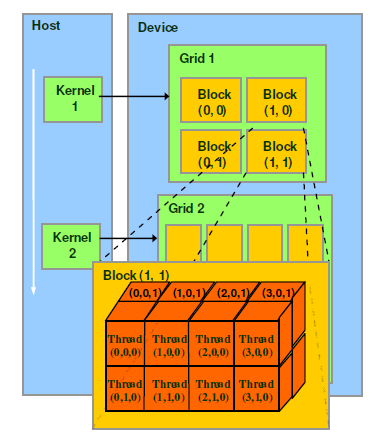
\includegraphics{cudathreads.png}
\caption{Image from \href{http://wiki.expertiza.ncsu.edu/images/7/7a/Cuda\_Fig2.png}{North Carolina State University}}\end{figure}

CUDA provides a handy type, \code{dim3} to keep track of these dimensions. You can
declare dimensions like this: \code{dim3 myDimensions(1,2,3);}, signifying the ranges on each
dimension.  Both blocks and grids
use this type even though grids are 2D.
To use a \code{dim3} as a grid dimension, leave out the last argument or set it to one.
Each device has it's own limit on the dimensions of blocks.
Run

\code{/usr/local/cuda/samples/1\_Utilities/deviceQuery/deviceQuery}

to find the limits for your device.


\section{Kernels}
\label{0-Introduction/Introduction:kernels}
CUDA threads are created by functions called kernels which must be \code{\_\_global\_\_}.
Kernels are launched with an extra set of parameters enclosed by \code{\textless{}\textless{}\textless{}} and
\code{\textgreater{}\textgreater{}\textgreater{}} the first argument is a \code{dim3} representing the grid dimensions and
the second is another \code{dim3} representing the block dimensions.
You can also use \code{int}s instead of \code{dim3}s, this will create a Nx1x1 grid.
After a kernel is launched, it creates the number of threads specified and runs each of them.
CUDA automatically waits for the devices to finish before you can access memory
using \code{cudaMemcpy()} although if you're using unified memory with
\code{cudaMallocManaged()} you will need to call \code{cudaDeviceSynchronize()} to
force the CPU to wait for the GPU.

\begin{Verbatim}[commandchars=\\\{\},numbers=left,firstnumber=1,stepnumber=1]
\PYG{n}{dim3} \PYG{n}{numBlocks}\PYG{p}{(}\PYG{l+m+mi}{8}\PYG{p}{,}\PYG{l+m+mi}{8}\PYG{p}{)}\PYG{p}{;}
\PYG{n}{dim3} \PYG{n}{threadsPerBlock}\PYG{p}{(}\PYG{l+m+mi}{8}\PYG{p}{,}\PYG{l+m+mi}{8}\PYG{p}{,}\PYG{l+m+mi}{8}\PYG{p}{)}\PYG{p}{;}
\PYG{n}{myKernel}\PYG{o}{\PYGZlt{}}\PYG{o}{\PYGZlt{}}\PYG{o}{\PYGZlt{}}\PYG{n}{numBlocks}\PYG{p}{,} \PYG{n}{threadsPerBlock}\PYG{o}{\PYGZgt{}}\PYG{o}{\PYGZgt{}}\PYG{o}{\PYGZgt{}}\PYG{p}{(}\PYG{n}{args}\PYG{p}{)}\PYG{p}{;}
\PYG{n}{myKernel}\PYG{o}{\PYGZlt{}}\PYG{o}{\PYGZlt{}}\PYG{o}{\PYGZlt{}}\PYG{l+m+mi}{16}\PYG{p}{,}\PYG{l+m+mi}{64}\PYG{o}{\PYGZgt{}}\PYG{o}{\PYGZgt{}}\PYG{o}{\PYGZgt{}}\PYG{p}{(}\PYG{n}{args}\PYG{p}{)}\PYG{p}{;}
\end{Verbatim}

Kernels have access to 4 variables that give information about a thread's location in the grid
\begin{enumerate}
\item {} 
\code{threadIdx.{[}xyz{]}} represents a thread's index along the given dimension.

\item {} 
\code{blockIdx.{[}xy{]}} represents a thread's block's index along the given dimension.

\item {} 
\code{blockDim.{[}xyz{]}} represents the number of threads per block in the given direction.

\item {} 
\code{gridDim.{[}xy{]}} represents the number of blocks in the given direction.

\end{enumerate}

By using these variables we can create a unique id for each thread indexed from 0 to N where N is the total number of threads.
For a one dimensional grid and a one dimesional block this formula is \code{blockIdx.x * blockDim.x + threadIdx.x}


\section{Compiling}
\label{0-Introduction/Introduction:compiling}
CUDA code is compiled with NVIDIA's own compiler nvcc.
You can still use makefiles like you do with regular c.
To make sure your code is taking full advantage of your device's capabilities use the flag
\code{-gencode arch=compute\_XX,code=sm\_XX} you can find the correct values of the Xs by running

\code{/usr/local/cuda/samples/1\_Utilities/deviceQuery/deviceQuery}

and using at the output of the CUDA capability line without the period.


\chapter{Vector Addition Lab}
\label{1-VectorAdd/VectorAdd:vector-addition-lab}\label{1-VectorAdd/VectorAdd::doc}
\begin{notice}{warning}{Warning:}
The Unified Memory parts of this lab may not work on your machine.
Run

\code{/usr/local/cuda/samples/1\_Utilities/deviceQuery/deviceQuery}

and check that your device's CUDA capability is \textgreater{}=
3.0 If the command gives you an error, you may need
to compile the samples like so

\begin{Verbatim}[commandchars=\\\{\}]
\PYG{n+nb}{cd} /usr/local/cuda/samples/1\PYGZus{}Utilities/deviceQuery
sudo make
./deviceQuery
\end{Verbatim}
\end{notice}


\section{Research Questions}
\label{1-VectorAdd/VectorAdd:research-questions}\begin{itemize}
\item {} 
For what size problem is the CUDA computation faster than the sequential
computation?

\item {} 
What effect does using Unified Memory have on the speed of our program?

\end{itemize}


\section{Getting started}
\label{1-VectorAdd/VectorAdd:getting-started}
Download and extract
\code{vectorAdd.tar.gz}
and extract it with \code{tar -xzvf vectorAdd.tar.gz}
Open vectorAdd.cu and vectorAdd6.cu and familiarize yourself with the code.
Compile and run the programs.

\begin{notice}{note}{Note:}
don't compile vectorAdd6.cu if your machine is incompatable
\end{notice}

Run the programs and see what happens.


\section{Exercise}
\label{1-VectorAdd/VectorAdd:exercise}

\subsection{Part One: cudaMemcpy}
\label{1-VectorAdd/VectorAdd:part-one-cudamemcpy}
Using omp\_get\_wtime() modify vectorAdd.cu so that it reports
\begin{enumerate}
\item {} 
The time required by the CUDA computation specifically
\begin{enumerate}
\item {} 
The time spent allocating A, B, and C

\item {} 
The time spent copying A and B from the Host to the device

\item {} 
The time spent computing the sum of A and B into C

\item {} 
The time spent copying C from the device to the host

\item {} 
The total time of the CUDA computation (i.e., the sum of a-d)

\end{enumerate}

\item {} 
The time required by the sequential computation

\end{enumerate}

None of these times should include any I/O so make sure you comment out
the printf() statements.

Use the Makefile to build your modified version of the program.
When it compiles successfully run it as follows:

\code{./vectorAdd}

The program's default array size is 50,000 elements

In a spreadsheet record and label your times in a column labeld 50,000. Which
is faster, the CUDA version or the CPU version?

Repeat this problem with a larger array. Run it again with 500,000 elements.

\code{./vectorAdd 500000}

Record your results. Repeat the process again wih 5,000,000 elements,
50,000,000 and 500,000,000 elements. How do these times compare?
Were you able to run all of them succesfully? If not why?

Create a line chart, with one line for the sequential code's
times and one line for the CUDA code's total times.
Your X-axis should be labeled with 50,000 500,000
5,000,000 and 50,000,000 your Y-axis should be the time.

Then create a ``stacked'' barchart of the CUDA times with the same X and Y axes
as your first chart.. For each X-axis value, this chart should ``stack''
the CUDA computation's
\begin{enumerate}
\item {} 
allocation time

\item {} 
host-to-device transfer time

\item {} 
computation time

\item {} 
device-to-host transfer time

\end{enumerate}

What observations can you make about the CUDA vs the sequential computations?
How much time does the CUDA computation spend transferring data compared to computing?
What is the answer to our first research question?


\subsection{Part Two: Unified Memory}
\label{1-VectorAdd/VectorAdd:part-two-unified-memory}
\begin{notice}{note}{Note:}
skip this section if your device is not compatable with Unified Memory.
\end{notice}

Using omp\_get\_wtime() modify vectorAdd6.cu so that it reports
\begin{enumerate}
\item {} 
The time spent allocating A, B, and C

\item {} 
The time spent computing the sum of A and B into C

\item {} 
The total time of the CUDA computation (i.e., the sum of a and b)

\end{enumerate}

Again, none of these times should include any I/O so make sure you comment out
the printf() statements.

Run your program using

\code{./vectorAdd6}

Record your results using 50,000 500,000 5,000,000 and
50,000,000 elements. How do these times compare?

Add this new data to the line chart and stacked bar charts from part one.
How does using unified memory compare to using \code{cudaMemcpy}?
What is the bottleneck for the \code{cudaMemcpy} version? What about
the unified memory version?


\chapter{More Exercises}
\label{2-MoreExercises/MoreExercises:more-exercises}\label{2-MoreExercises/MoreExercises::doc}
\begin{notice}{note}{Note:}
If your device is incompatable with CUDA 6, don't edit or build the files ending with a 6
\end{notice}


\section{Exercise II: Vector Multiplication}
\label{2-MoreExercises/MoreExercises:exercise-ii-vector-multiplication}
Let's try the same research questions, but using a more expensive operation like multiplication.

In your vectorAdd directory, run
\begin{quote}

\code{make clean}
\end{quote}

to remove the binary. Then run
\begin{quote}

\code{cd ..}

\code{cp -r vectorAdd vectorMult}
\end{quote}

to create a copy of your vectorAdd folder named vectorMult. Inside there,
rename vectorAdd.cu and vectorAdd6.cu vectorMult.cu and vectorMult6.cu
and modify the Makefile to build vectorMult and vectorMult 6 instead of vectorAdd and vectorAdd6.
Then edit vectorMult.cu and vectorMult6.cu so that they store the
product of A{[}i{]} times B{[}i{]} in C{[}i{]} instead of the sum.
Note that for both programs you will need to change:
\begin{itemize}
\item {} 
The CUDA version.

\item {} 
The verification test for the CUDA version.

\item {} 
The sequential version.

\item {} 
The verification test for the sequential version.

\end{itemize}

Then build vectorMult and vectorMult6 and run them using 50,000
500,000 5,000,000 and 50,000,000 element arrays.
Record the timings for each of these in your spreadsheet,
and create charts to help us visualize the results
like you did with the vectorAdd programs.

What are the answers to our research questions?
How do your results compare to those of Exercise I?


\section{Exercise III: Vector Square Root}
\label{2-MoreExercises/MoreExercises:exercise-iii-vector-square-root}
Let's try the same research questions, but this time using an even
more expensive operation AND reducing the amount of data we're transferring.
Calculating a square root is a more expensive operation than multiplication, so let's try that.

As in Exercise II, clean and make a copy of your vectorMult folder named vectorRoot.
Inside it, rename vectorMult.cu and vectorMult6.cu vectorRoot.cu and vectorRoot6.cu respectively.
Modify the Makefile to build vectorRoot and vectorRoot6.

Then edit vectorRoot.cu and vectorRoot6.cu so they compute the square root of A{[}i{]} in C{[}i{]}.

Then build vectorRoot and vectorRoot6 and run them using 50,000
500,000 5,000,000 and 50,000,000 element arrays.
As before, record the timings for each of these in your
spreadsheet, and create charts to help us visualize the results.

What are the answers to our research questions?
How do these results compare to those of Exercises I and II?


\section{Exercise IV: Vector Square}
\label{2-MoreExercises/MoreExercises:exercise-iv-vector-square}
Let's try the same research questions one more time.
This time, we will use a less expensive operation than square root,
but keep the amount of data we're transferring the same.

As in Part III, clean and make a copy of your vectorRoot folder named vectorSquare.
Inside it, rename vectorRoot.cu and vectorRoot6.cu vectorSquare.cu and vectorSquare6.cu respectively.
Modify the Makefile to build vectorSquare and vectorSquare6.

Then edit vectorSquare.cu and vectorSquare6.cu so they compute the square of A{[}i{]} in C{[}i{]}.

Then build vectorSquare and vectorSquare6 and run them using 50,000
500,000 5,000,000 and 50,000,000 array elements.
As before, record the timings for each of these in your spreadsheet,
and create charts to help us visualize the results.

What are the answers to our research questions?
How do your results compare to those of the previous parts?



\renewcommand{\indexname}{Index}
\printindex
\end{document}
